\documentclass{beamer}
\usetheme[hideothersubsections]{Berkeley}
\usepackage{tikz}
\usetikzlibrary{fadings}
\usetikzlibrary{positioning}
\usepackage{listings}
\usepackage{array}
\usepackage[export]{adjustbox}
\newcolumntype{L}{>{\centering\arraybackslash}m{3cm}}
\makeatletter
\setbeamertemplate{sidebar \beamer@sidebarside}%{sidebar theme}
  {
    \beamer@tempdim=\beamer@sidebarwidth%
    \advance\beamer@tempdim by -6pt%
    \insertverticalnavigation{\beamer@sidebarwidth}%
    \vfill
    \ifx\beamer@sidebarside\beamer@lefttext%
    \else%
      \usebeamercolor{normal text}%
      \llap{\usebeamertemplate***{navigation symbols}\hskip0.1cm}%
      \vskip2pt%
    \fi%
  }%
\makeatother


\title{Automatic Detection of Pseudo-Tested Methods in a Test Suite Using Fault Injection}
\author{Nicholas Tocci}
\date{\today}

\begin{document}
%%%%%%%%%%%% Introduction %%%%%%%%%%%%%%%%%%%%%%%%%%%%%%%%%%%%%%%%%%%%%%%%%%%
\section{Introduction}
\begin{frame}
	\frametitle{Introduction}
	\titlepage
\end{frame}
%%%%%%%%%%%% Problem %%%%%%%%%%%%%%%%%%%%%%%%%%%%%%%%%%%%%%%%%%%%%%%%%%%
\section{Problem}
\label{sec:problem}
%%%%%%%%%%%% Slide %%%%%%%%%%%%%%%%%%%%%%%%%%%%%%%%%%%%%%%%%%%%%%%%%%%
\begin{frame}
	\frametitle{Problem}
	\begin{center}
		\huge{How can we know if our test suites are adequate?}

		
\includegraphics[scale = .25]{images/thumb}
	\end{center}
\end{frame}

% Beginning of Current Metrics
\subsection{Coverage}
%%%%%%%%%%%% Slide %%%%%%%%%%%%%%%%%%%%%%%%%%%%%%%%%%%%%%%%%%%%%%%%%%%
\begin{frame}
	\frametitle{Coverage}
		\begin{center}
			\huge{Coverage}

			
\includegraphics[scale = 0.25]{images/percent.png}

			\textbf{\textit{Def}}: \% of a system that has been tested.
		\end{center}




\end{frame}

\subsubsection{Calculation}
%
% This sections will explain why Passing Test Cases do not indicate a good Test Suite.
%
\begin{frame}
	\frametitle{Calculation}
	\begin{center}
		\begin{equation*}
			Coverage = \frac{Number of Tested Methods}{Total Number of Methods}
		\end{equation*}
	\end{center}
\end{frame}

\subsubsection{Coverage vs Adequate Coverage}
%
% This sections will explain why High Coverage can mislead a developer.
%
\begin{frame}
	\frametitle{High Coverage}
		\begin{center}
			
\includegraphics[scale = .15]{images/percentEquals}
		\end{center}
\end{frame}


\section{Pseudo-tested Methods}
\label{sec:pseudo-tested methods}
\begin{frame}
	\frametitle{Pseudo-tested Methods}
	\begin{center}
    \huge{Pseudo-tested Methods}
  \end{center}
\end{frame}

\subsection{Defintion}
\begin{frame}
  \frametitle{Definition}
    \begin{center}
      \textbf{What is a Pseudo-tested Method?}

      \vspace{10mm}
      
\includegraphics{images/passing}

      \vspace{10mm}
      \textbf{\textit{Def}}: It will never fail.
    \end{center}
\end{frame}

\subsection{Detection}
\begin{frame}
  \frametitle{Detection}
    \begin{center}
      \textbf{How Can We Detect Pseudo-tested Methods}

			\vspace{20mm}
			\textbf{It is harder than you think!}

    \end{center}
\end{frame}

% \begin{frame}
% \begin{figure}[t!]
% \begin{lstlisting}[language = Python, numbers = left, frame = single, caption = Example of a pseudo-tested method]
% numbers.py:
%   def numberOrder(n):
%     numbersSorted = sorted(n)
%     return numbersSorted
%
%
% test_numbers.py:
%   def test_numbers_ordered():
%     numbers = {1,3,2,4}
%     sortedNumbers = {1,2,3,4}
%     orderedNumbers = numberOrder(numbers)
%     assert numbers == sortedNumbers
% \end{lstlisting}
% \end{figure}
% \end{frame}


\section{Function-Fiasco}
\label{sec:function-fiasco}
\subsection{What is Function-Fiasco}
\begin{frame}
  \frametitle{What is Function-Fiasco}
    \begin{center}
      \huge{\textbf{A Pseudo-tested method detection tool}}
    \end{center}
\end{frame}

\subsection{Flow}
\begin{frame}
  \frametitle{Flow to system}
    \begin{center}
      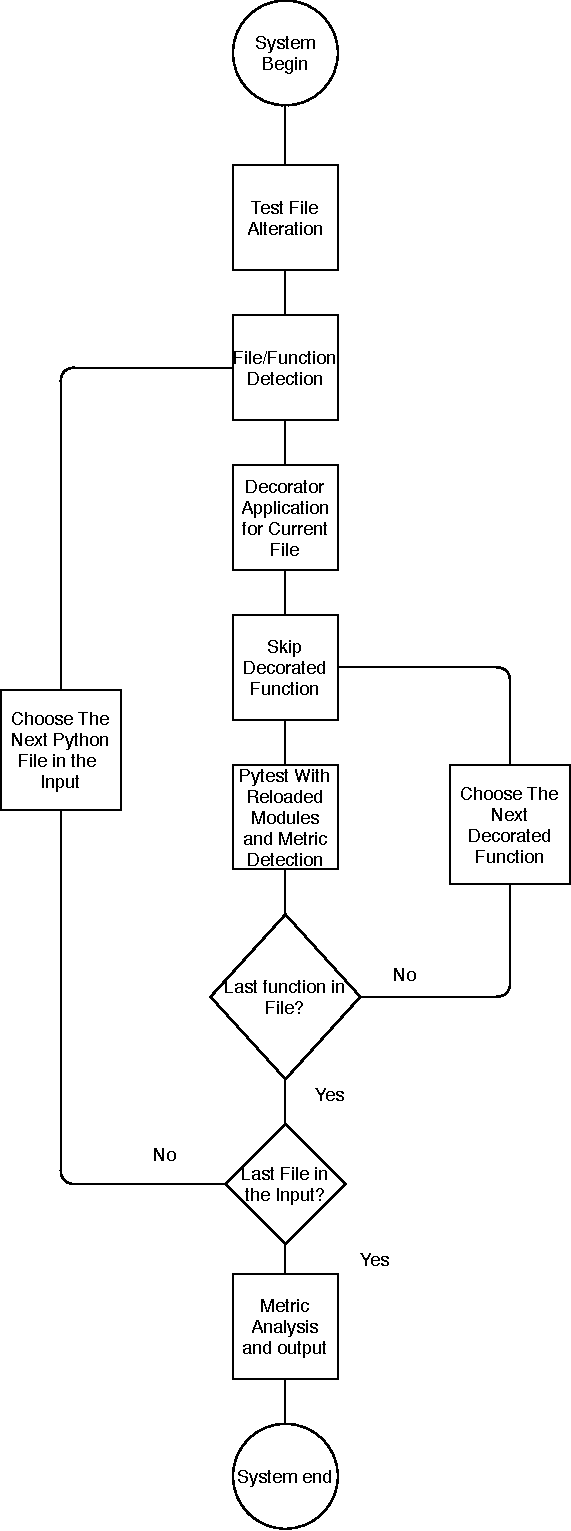
\includegraphics[scale = .25]{images/flow1}
    \end{center}
\end{frame}


\section{Evaluation Strategy}
\label{sec:Evaluation Strategy}
\subsection{Coverage Calculation}
\begin{frame}
\frametitle{Coverage Calculation}
\begin{center}
  \begin{equation*}
    Coverage = \frac{Number of Tested Methods}{Total Number of Methods}
  \end{equation*}
\end{center}
\end{frame}

\begin{frame}
  \frametitle{Coverage Example}
  \begin{center}

  \begin{table}[htbp]
  %   \centering
   \resizebox{6.5cm}{!}{%
    \begin{tabular}{|c|c|c|c|c|c|}
      \hline
  %
      \bf NUMM     & \bf NUMTM & \bf Coverage \\ \hline\hline
      40  & 25  & 62.5\%  \\ \hline
  %
  %
    \end{tabular}%
    }

  \end{table}

  \end{center}
\end{frame}

\subsection{Truly-Tested-Method Calculation}
\begin{frame}
  \frametitle{Truly-Tested-Method Calculation}
  \begin{itemize}
    \item \textbf{Number of Truly-Tested-Methods = NUMTTM}

    \item \textbf{Number of Tested Methods = NUMTM}

    \item \textbf{Number of Pseudo-tested Methods = NUMPTM}
  \end{itemize}

  \begin{center}
    \begin{equation*}
      NUMTTM = NUMTM - NUMPTM
    \end{equation*}
  \end{center}
\end{frame}

\begin{frame}
  \frametitle{Truly-Tested-Method Example}
  \begin{center}

  \begin{table}[htbp]
  %   \centering
   \resizebox{6.5cm}{!}{%
    \begin{tabular}{|c|c|c|c|c|c|}
      \hline
  %
      \bf NUMTM     & \bf NUMPTM & \bf NUMTTM \\ \hline\hline
      25  & 3  & 22  \\ \hline
  %
  %
    \end{tabular}%
    }

  \end{table}

  \end{center}
\end{frame}

\begin{frame}
\frametitle{Adequate-Coverage Calculation}
\begin{center}
  \begin{equation*}
    AC = \frac{Number of TrulyTested Methods}{Total Number of Methods}
  \end{equation*}
\end{center}
\end{frame}

\subsection{Metrics Produced}
\begin{frame}
  \frametitle{Output}
    \begin{center}

    \begin{table}[htbp]
      \centering
    \resizebox{9.5cm}{!}{%
      \begin{tabular}{|c|c|c|c|c|c|}
        \hline

        \bf NUMM     & \bf NUMTM & \bf Coverage & \bf NUMPTM & \bf NUMTTM & \bf AC\\ \hline\hline
        40  & 25  & 62.5\%  & 3 & 22 &  55\%  \\ \hline


      \end{tabular}%
      }

    \end{table}

    \end{center}
\end{frame}


\section{Conclusion}
\label{sec:Conclusion}
\subsection{What is Function-Fiasco}
\begin{frame}
  \frametitle{What is Function-Fiasco}
    \begin{center}
      \huge{\textbf{A Pseudo-tested method detection tool}}
    \end{center}
\end{frame}

\end{document}
